\documentclass[final]{beamer}
\usepackage[orientation=portrait,size=a0,scale=1.3]{beamerposter}
\usepackage[icelandic]{babel}
\usepackage[T1]{fontenc}

\usepackage{lmodern}
\usepackage{fontspec}

\usepackage{tcolorbox}
\usepackage{hyperref} 


\hypersetup{pdfencoding=auto}
\setmainfont{Arial} 
\usetheme{vonmaster}
\graphicspath{{./figs/}{../report/figs/}}

%\beamertemplategridbackground[1cm]% Display a grid to help align images

\title{Nútímaleg vefkennsla í notkun gagnasafna með opnum hugbúnaði} 
\author{Eiríkur Ernir Þorsteinsson} 
\institute{Iðnaðarverkfræði-, vélaverkfræði- og tölvunarfræðideild} 
\newcommand{\insertinstructor}{Hjálmtýr Hafsteinsson}  % Not official, but provided for consistency
\date{Maí 2017}

\begin{document}
\begin{frame}
\begin{tcolorbox}[standard jigsaw, height=97cm, colframe=orange, opacityback=0, sharp corners=all]
\begin{columns}[t]

\begin{column}{.47\linewidth}

\begin{block}{Markmið}
    
\end{block}

\begin{block}{Opinn kóði, opið kennsluefni}
    Mikilvægt að allt sé opið og næs
\end{block}

\begin{block}{Ólínuleg framvinda}
    
\end{block}

\begin{block}{Sérhæfðar Markdown-viðbætur}
\end{block}

\begin{block}{Markviss textaframsetning}
    
\end{block}
\end{column}

\begin{column}{.47\linewidth}

\begin{block}{SQLite í minni}
Nemendafyrirspurnir eru keyrðar á SQLite gagnagrunnstilvikum í aðalminni vefþjónsins. Þegar meta skal skipun er tómur gagnagrunnur búinn til í minni, gerðarlýsingin sett upp,nemendafyrirspurnin keyrð ásamt samanburðarfyrirspurn og niðurstöðumengin borin saman.
\begin{figure}
    \caption{Keyrsla nemendafyrirspurnar}
    \begin{center}
    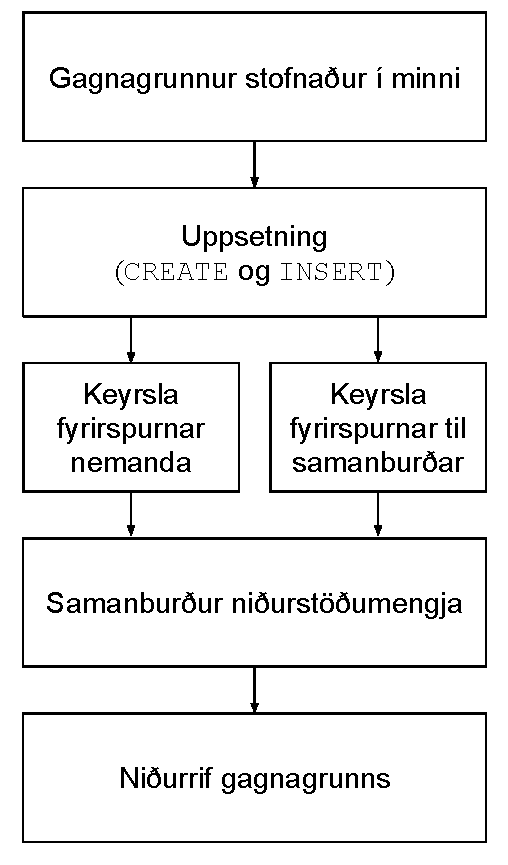
\includegraphics[width=\linewidth]{keyrsla-fyrirspurnar}
\end{center}
\end{figure}

Eftir að samanburði lýkur er gagnagrunnstilvikinu eytt.
\end{block}
\end{column}

\end{columns}
\end{tcolorbox}
\end{frame}

\end{document}